\documentclass[11pt,letterpaper]{article}
\usepackage[margin=1in]{geometry}
\usepackage{fontspec}
\usepackage[nopatch=footnote]{microtype}
\usepackage{booktabs,graphicx,amsmath,array,float}
\usepackage[round,authoryear]{natbib}
\usepackage[font=small,labelfont=bf]{caption}
\usepackage[hidelinks]{hyperref}
\usepackage{xurl,setspace}
\setstretch{1.15}
\setlength{\emergencystretch}{2em}
\graphicspath{{../figs/}}
\newcommand{\RosterOriginals}{2,394}
\newcommand{\EligibleOriginals}{1,068}
\newcommand{\EligibleSuccessful}{568}
\newcommand{\EligibleFailed}{500}
\newcommand{\OutsideSupport}{81}
\newcommand{\OutsidePercent}{35.7}
\newcommand{\ReportClusters}{142}
\newcommand{\LargestReport}{64}
\newcommand{\DistinctControls}{748}
\newcommand{\MaximumReuse}{21}
\newcommand{\StoppedHistories}{10,121}
\newcommand{\CitationsThrough}{2025}
\newcommand{\CommonHistoryN}{82}
\newcommand{\ThreeHistoryN}{282}
\newcommand{\FiveHistoryN}{227}
\newcommand{\EightHistoryN}{109}
\newcommand{\TenHistoryN}{82}
\newcommand{\FirstEventYear}{1975}
\newcommand{\LastEventYear}{2022}
\newcommand{\MainSuccessfulN}{115}
\newcommand{\MainSuccessfulEstimate}{\ensuremath{+2.05}}
\newcommand{\MainSuccessfulInterval}{\ensuremath{[-1.42,\,5.52]}}
\newcommand{\MainFailedN}{112}
\newcommand{\MainFailedEstimate}{\ensuremath{+3.02}}
\newcommand{\MainFailedInterval}{\ensuremath{[-0.65,\,6.69]}}
\newcommand{\MainDifferenceN}{227}
\newcommand{\MainDifferenceEstimate}{\ensuremath{+0.97}}
\newcommand{\MainDifferenceInterval}{\ensuremath{[-3.67,\,5.61]}}
\newcommand{\ShortSuccessfulN}{180}
\newcommand{\ShortSuccessfulEstimate}{\ensuremath{+1.57}}
\newcommand{\ShortSuccessfulInterval}{\ensuremath{[-0.24,\,3.38]}}
\newcommand{\ShortFailedN}{185}
\newcommand{\ShortFailedEstimate}{\ensuremath{+2.31}}
\newcommand{\ShortFailedInterval}{\ensuremath{[0.13,\,4.49]}}
\newcommand{\ShortDifferenceN}{365}
\newcommand{\ShortDifferenceEstimate}{\ensuremath{+0.74}}
\newcommand{\ShortDifferenceInterval}{\ensuremath{[-1.81,\,3.29]}}
\newcommand{\SuccessfulPre}{27.1}
\newcommand{\SuccessfulControlPre}{9.2}
\newcommand{\SuccessfulPlaceboN}{64}
\newcommand{\SuccessfulPlacebo}{\ensuremath{+5.48}}
\newcommand{\FailedPre}{19.5}
\newcommand{\FailedControlPre}{12.1}
\newcommand{\FailedPlaceboN}{56}
\newcommand{\FailedPlacebo}{\ensuremath{+1.16}}

\title{Do citations respond to replication results?\thanks{Data and code: \url{https://github.com/recite/i4r_response}. This research note reports an incomplete collection snapshot; the estimates are exploratory.}}
\author{Gaurav Sood}
\date{}
\hypersetup{pdfauthor={Gaurav Sood},pdftitle={Do citations respond to replication results?}}
\widowpenalty=10000
\clubpenalty=10000
\renewcommand{\topfraction}{.9}
\renewcommand{\textfraction}{.1}
\renewcommand{\floatpagefraction}{.8}
\begin{document}
\maketitle
\begin{abstract}
\noindent Citations may respond to a replication report without reflecting whether its findings were favorable. We compare changes in annual citations to replicated papers with changes to papers from the same journal and publication year, matched on prior citations. Among \MainDifferenceN{} originals matched on five pre-report years, the matched change is \MainSuccessfulEstimate{} citations per year following a successful replication and \MainFailedEstimate{} following a failed replication. The failed-minus-successful difference is \MainDifferenceEstimate{} (95\% interval \MainDifferenceInterval{}). This interval permits differences in either direction. Collection is incomplete, many originals are more highly cited than their controls, and held-out pre-period changes favor the originals. These estimates therefore do not establish a causal effect of replication reports. They describe citation responses in an observed subset and identify the comparison and measurement problems that must be resolved before interpreting continued citation as a failure of scientific correction.
\end{abstract}

\section{Citation responses and scientific correction}
Failed replications are not followed by a clearly different citation response from successful replications in the comparisons available here. The estimated difference is \MainDifferenceEstimate{} citations per paper per year, with a 95\% interval of \MainDifferenceInterval{}. The interval is too wide to treat the two responses as equivalent, and the comparison papers do not closely reproduce the originals' citation histories.

Replication can change the evidential basis for a finding. If later researchers learn that a finding does not replicate, they may stop relying on it, qualify their use of it, or defend it against the challenge. Citation counts capture only part of that response. A citation can endorse a claim, criticize it, or use a method unrelated to the challenged finding. A replication report can also draw attention to a paper and increase citations while reducing confidence in its conclusion.

Earlier studies do not give a single answer about citation penalties. Nonreplicable papers in prominent replication projects received more citations than replicable papers, and the gap persisted after replication \citep{serra2021}. Analyses of psychology replications found little evidence of adjustment, or small and uncertain differences between successful and failed replications \citep{schafmeister2021,vonhippel2022}. Another analysis found declines after failed replications \citep{clark2023}. Citation-context studies also show why counts alone are insufficient: favorable use can persist alongside some increase in criticism \citep{hardwicke2021}. Continued citation and a citation penalty can coexist.

This note extends the comparison to a common registry of replication attempts. It uses the same event-selection and matching rules for successful and failed replications and reports both the estimated responses and the quality of the comparisons. The contribution at this stage is a reproducible comparison across recorded assessments, rather than a new demonstration that challenged research continues to be cited. The current data cannot distinguish continued attention from continued reliance on the challenged result.

\section{Data and research design}
The FORRT Library of Reproduction and Replication Attempts (FLoRA) links original papers to reports and records replication authors' descriptions of their outcomes \citep{flora2026}. We retain those source labels. A failed replication is not a finding that the original paper is false in every respect, and success criteria differ across reports. I4R records supply additional assessment histories and help exclude already assessed papers from the control pool. The binary outcome analysis here uses FLoRA replication labels; it is not an estimate of the response to I4R computational reproductions.

We verify article identities, titles, types, journals, and publication dates with Crossref and OpenAlex metadata. For each original, we select the earliest recorded journal-report year before filtering on outcome. Conflicting outcomes in that year receive a mixed label. An unverified report that could precede or coincide with the selected report prevents confident assignment. This procedure avoids selecting a convenient later failure after an earlier success. Journal publication is observable, but a preprint, presentation, or other disclosure may have made the result public earlier.

The roster contains \RosterOriginals{} originals; \EligibleOriginals{} pass the event and metadata screens for matching, including \EligibleSuccessful{} with successful and \EligibleFailed{} with failed replications. These are not all completed comparisons. The primary five-year matching analysis contains \MainSuccessfulN{} successful and \MainFailedN{} failed originals, with report years from \FirstEventYear{} to \LastEventYear{}. A shorter window contains \ShortDifferenceN{} originals. The samples overlap and must not be added. Collection stopped under its spending limit with \StoppedHistories{} requested histories still unavailable; missing histories are never coded as zero. This is a collection constraint, not evidence that those histories do not exist.

Annual citations count OpenAlex article and review works citing a paper, by the citing work's publication year, through \CitationsThrough{} \citep{openalex2022}. Complete histories must reconcile with the retrieved total. We compare the mean of the three full years before the report with the mean of the three full years after it, excluding the report year. The shorter window uses two years before and one after. Both originals and controls must have been published before the first baseline year.

Each comparison starts with a fixed seeded sample of up to twenty papers from the original's journal and indexed publication year. We exclude known assessed originals and assessment reports, nonresearch items, current retraction flags, and unresolved metadata conflicts. Current retraction status is a retrospective restriction; it does not establish that retained controls escaped every criticism. Matching within journal and year follows an established approach to citation responses \citep{furman2012,schafmeister2021}.

We use five pre-report years to select up to five controls with the smallest average squared distance in baseline $\log(1+\text{citations})$, scaling each year's difference by the candidate pool's population standard deviation and omitting constant coordinates. Ties are resolved by paper identifier after rounding distances to ten decimal places. Post-report outcomes do not enter selection. A missing eligible candidate's baseline blocks matching; missing follow-up for a selected control blocks the comparison rather than prompting replacement. There is no distance caliper, so the nearest available controls can still be poor matches.

For original $i$ with controls $C_i$, the comparison is
\begin{equation}
 d_i = \left(\overline{Y}_{i,\mathrm{post}}-\overline{Y}_{i,\mathrm{pre}}\right)
 -\frac{1}{|C_i|}\sum_{j\in C_i}
 \left(\overline{Y}_{j,\mathrm{post}}-\overline{Y}_{j,\mathrm{pre}}\right).
\end{equation}
We average $d_i$ with equal weight per original within each replication-outcome group. The difference between these averages is the failed-minus-successful contrast. All quantities are in citations per paper per year. They are neither percentage changes nor effects for the population of all published research.

For uncertainty, a weighted regression of change scores on original-by-outcome indicators and comparison fixed effects reproduces these group means. Each original has weight one and its controls jointly have weight one. We cluster by physical paper, because controls can be reused, and by connected report bundle, because a report can assess several originals. Intervals use a cluster correction, a correction for nonnested fixed effects, and a $t$ critical value based on the smaller cluster count minus one. They condition on the selected matches and source labels. Interpreting the averages as effects on assessed papers would additionally require parallel counterfactual trends, no anticipation, and no differential coincident shocks. Comparing the averages does not identify the causal effect of failure rather than success.

\section{Results and comparison quality}
Both outcome groups have positive point estimates of matched changes (Figure~\ref{fig:response}). The successful group changes by \MainSuccessfulEstimate{} citations per year (95\% interval \MainSuccessfulInterval{}); the failed group changes by \MainFailedEstimate{} (\MainFailedInterval{}). Their difference, \MainDifferenceEstimate{}, is uncertain. A shorter window, also using only two pre-report years for matching, gives a failed-minus-successful difference of \ShortDifferenceEstimate{} (\ShortDifferenceInterval{}). These estimates do not show that researchers ignore replication results, nor do the positive changes establish that reports increase citations.

\begin{figure}[htbp]
\centering
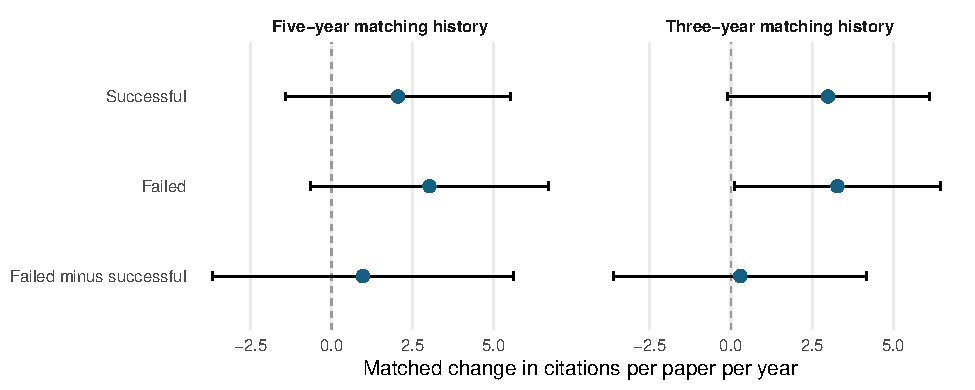
\includegraphics[width=\linewidth]{citation_response.pdf}
\caption{Matched changes after successful and failed replications. Points are mean original-minus-control changes and their failed-minus-successful difference; bars are 95\% intervals clustered by physical paper and connected report bundle, conditional on matches and labels. Five-year matching includes \MainDifferenceN{} originals and three-year matching includes \ThreeHistoryN{}. Both use the last three pre-report years and first three post-report years to measure change, omitting the report year. Panels share an axis, and zero marks no matched change or no difference between outcome groups.}
\label{fig:response}
\end{figure}

The originals are substantially more highly cited than their controls in the last three years before the report (Figure~\ref{fig:paths}). Successful originals average \SuccessfulPre{} annual citations against \SuccessfulControlPre{} for their controls; failed originals average \FailedPre{} against \FailedControlPre{}. Controls' citations fall slightly after the report while originals' citations rise (Table~\ref{tab:diagnostics}). Level differences alone do not refute parallel trends, but they show that the sampled controls do not closely approximate these originals. In \OutsideSupport{} of \MainDifferenceN{} comparisons (\OutsidePercent\%), an original lies outside its entire candidate pool's citation range in at least one of the five matching years.

\begin{figure}[htbp]
\centering
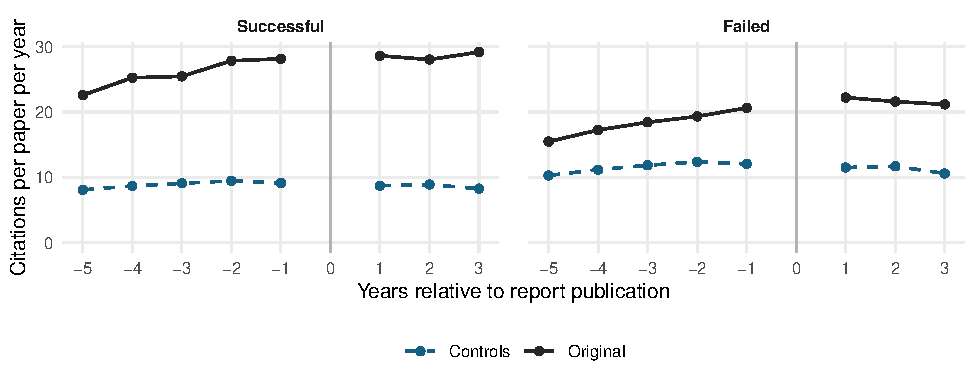
\includegraphics[width=\linewidth]{citation_paths.pdf}
\caption{Observed citation paths in the primary five-year matching sample, by replication outcome. Each original has equal weight; its controls first receive equal weight within its comparison. Lines show descriptive means for the same \MainSuccessfulN{} successful and \MainFailedN{} failed originals across all plotted years, without inferential intervals. Both panels use common axes. The report year is omitted and lines break there. These are observed paths, not estimated counterfactuals.}
\label{fig:paths}
\end{figure}

A held-out comparison also favors originals before the matching window. Using the two preceding years, the mean original-minus-control annual change is \SuccessfulPlacebo{} for \SuccessfulPlaceboN{} successful originals and \FailedPlacebo{} for \FailedPlaceboN{} failed originals. These are descriptive diagnostics on older subsets, not formal tests of parallel trends. Their direction is consistent with preexisting differences in citation growth that could contribute to the positive post-report contrasts.

Report concentration and control reuse also matter. The main sample has \ReportClusters{} connected report bundles, with \LargestReport{} originals in the largest bundle, and \DistinctControls{} distinct controls, one used in as many as \MaximumReuse{} comparisons. Clustering addresses dependence in estimated uncertainty but cannot repair weak comparisons. Excluding the largest report, excluding later or prior other assessments, and restricting originals to their candidate pool's range leaves the failed-minus-successful intervals spanning zero (Table~\ref{tab:sensitivity}). Each restriction changes the population being described.

\section{What the comparison establishes}
The observed subset does not provide a precise distinction between citation responses to successful and failed replications. Incomplete collection also prevents treating it as representative of eligible assessed papers. Supplementary Section~\ref{sec:design} specifies longer histories, full same-journal/year candidate pools, and dated control eligibility. Finishing collection will expand the comparison, but will not by itself resolve the large baseline gaps, earlier disclosure, or differences in why particular papers were replicated.

A stronger claim about scientific correction requires observing how later papers use the challenged finding. The relevant unit is a claim in a citing passage: does the passage rely on that finding as evidence, acknowledge the replication, qualify its use, or offer a defense? Existing citation-context research provides a precedent for that distinction \citep{hardwicke2021}. A further measurement step is a before-and-after sample of accessible citing texts, with claim-specific coding checked against human judgments. No completed context ratings are reported here. Even an unqualified citation cannot establish that its author knew of the replication or that every use of the original paper was unwarranted.

\paragraph{Data and code.} The public repository contains the pinned source references, metadata, collected histories, analysis code, and generated exhibits. Run \texttt{make restore} and \texttt{make paper} with R and XeLaTeX to rebuild the note; \texttt{make check} verifies the analysis and compiles the manuscript. Data attribution and reuse terms are in \texttt{data/README.md}. Every reported estimate and sample count is generated from the analysis rather than copied into the manuscript.

\clearpage
\begingroup
\small
\bibliographystyle{plainnat}
\bibliography{references}
\endgroup

\clearpage
\appendix
\section{Diagnostics and sensitivity}
\begin{table}[H]
\centering
\caption{Citation levels and comparison quality in the primary five-year matching sample.}
\label{tab:diagnostics}
\small
\begin{tabular}{lrr}
\toprule
Quantity & Successful & Failed \\
\midrule
Original papers & 115 & 112 \\
Original citations before report (per year) & 27.14 & 19.46 \\
Original citations after report (per year) & 28.59 & 21.65 \\
Control citations before report (per year) & 9.25 & 12.10 \\
Control citations after report (per year) & 8.64 & 11.27 \\
Outside candidate range (papers) & 38 & 43 \\
With held-out pre-period data (papers) & 64 & 56 \\
Held-out difference in annual changes & 5.48 & 1.16 \\
\bottomrule
\end{tabular}

\par\smallskip\begin{minipage}{\linewidth}\footnotesize
Pre- and post-report levels average the last three years before and first three after, omitting the report year. Control levels average within comparison before averaging across originals. Outside-range counts refer to at least one baseline year outside the full eligible candidate pool's range during the five matching years. The held-out diagnostic compares changes between the two years preceding the matching window; its sample requires sufficiently old originals and controls with complete histories. It has no reported inferential interval.
\end{minipage}
\end{table}

\begin{table}[H]
\centering
\caption{Failed-minus-successful contrasts under sample restrictions.}
\label{tab:sensitivity}
\small
\begin{tabular}{lrrr}
\toprule
Window and sample & Originals & Difference & 95\% interval \\
\midrule
\multicolumn{4}{l}{\textit{Five-year matching history}} \\
All completed comparisons & 227 & \ensuremath{+0.97} & \ensuremath{[-3.67,\,5.61]} \\
Omit largest report & 163 & \ensuremath{+2.46} & \ensuremath{[-3.48,\,8.40]} \\
No later assessment & 217 & \ensuremath{+0.16} & \ensuremath{[-4.39,\,4.72]} \\
No prior other assessment & 226 & \ensuremath{+0.95} & \ensuremath{[-3.71,\,5.61]} \\
Within candidate range & 146 & \ensuremath{+1.78} & \ensuremath{[-3.27,\,6.83]} \\
\addlinespace
\multicolumn{4}{l}{\textit{Three-year matching history}} \\
All completed comparisons & 282 & \ensuremath{+0.29} & \ensuremath{[-3.62,\,4.19]} \\
Omit largest report & 218 & \ensuremath{+1.22} & \ensuremath{[-3.52,\,5.96]} \\
No later assessment & 269 & \ensuremath{-0.19} & \ensuremath{[-4.17,\,3.78]} \\
No prior other assessment & 281 & \ensuremath{+0.27} & \ensuremath{[-3.64,\,4.19]} \\
Within candidate range & 195 & \ensuremath{+0.58} & \ensuremath{[-2.74,\,3.90]} \\
\addlinespace
\multicolumn{4}{l}{\textit{Two before / one after}} \\
All completed comparisons & 365 & \ensuremath{+0.74} & \ensuremath{[-1.81,\,3.29]} \\
Omit largest report & 301 & \ensuremath{+1.23} & \ensuremath{[-1.77,\,4.23]} \\
No later assessment & 359 & \ensuremath{+0.56} & \ensuremath{[-2.03,\,3.16]} \\
No prior other assessment & 364 & \ensuremath{+0.75} & \ensuremath{[-1.81,\,3.31]} \\
Within candidate range & 274 & \ensuremath{+0.63} & \ensuremath{[-1.74,\,3.00]} \\
\addlinespace
\bottomrule
\end{tabular}

\par\smallskip\begin{minipage}{\linewidth}\footnotesize
Differences and intervals are in citations per paper per year. Intervals use two-way paper/report clustering as in Figure~\ref{fig:response}. ``No later assessment'' excludes originals with another recorded assessment within the outcome window. ``No prior other assessment'' excludes flags for earlier reproduction or I4R overlap. ``Within candidate range'' excludes originals outside the pool's range in any baseline year. These are different analytic populations, not repeated estimates on a fixed sample.
\end{minipage}
\end{table}
\clearpage
\section{Choice of pre-period and controls}
\label{sec:design}
The target is the average effect of a replication report on citations to the papers assessed, separately by its source-coded outcome. For report cohort $g$, outcome label $s$, and event time $k$, the target is
\[
 \operatorname{ATT}_{s}(g,k)
 = E\!\left[Y_{i,g+k}(g)-Y_{i,g+k}(\infty)
       \mid G_i=g,\ S_i=s,\ i\in\mathcal{S}\right].
\]
Here $\mathcal{S}$ is the set of completed comparisons under the stated matching specification. The corresponding target over all eligible originals would require completed collection or additional assumptions about selection into this subset. The reported three-year response averages $k=1,2,3$, then averages over originals with equal weight. $Y(g)$ is the citation path with a report at $g$ and $Y(\infty)$ the path without that report. Cohort aggregation should weight original papers equally. The difference between outcome-specific ATTs describes different groups of papers; it is not the effect of assigning a failed rather than successful outcome. The implemented matched contrasts estimate these targets only under the identifying assumptions in the main text.

\subsection{Retain long histories; separate matching from measurement}
We retain citation histories from indexed publication through \CitationsThrough{}. The primary specification uses five complete pre-report years to choose controls, while measuring change between the last three pre-report years and the first three post-report years. The outcome contrast stays fixed when the matching history changes. Three-year matching is a sensitivity; eight- and ten-year matching examine older originals.

Table~\ref{tab:history} separates availability from age. Longer baselines exclude papers assessed soon after publication even if collection is complete. Five years retains \FiveHistoryN{} comparisons; eight and ten retain \EightHistoryN{} and \TenHistoryN{}. We selected five years after inspecting these coverage counts and before inspecting the longer-history effect estimates. The original three-year estimates had already been examined. This is an exploratory design revision, not a preregistration.

\begin{table}[H]
\centering
\caption{Availability of longer matching histories.}
\label{tab:history}
\small
\begin{tabular}{lrrrr}
\toprule
Matching years & Old enough & Available & Common sample & Missing baseline \\
\midrule
3 & 961 & 282 & 82 & 477 \\
5 & 729 & 227 & 82 & 338 \\
8 & 385 & 109 & 82 & 186 \\
10 & 278 & 82 & 82 & 131 \\
\bottomrule
\end{tabular}

\par\smallskip\begin{minipage}{\linewidth}\footnotesize
The starting roster has \EligibleOriginals{} eligible originals. Old enough applies only the original's publication-age condition, not follow-up or controls. Available additionally requires a complete pool, baseline histories, and selected follow-up. Missing baseline counts otherwise feasible comparisons blocked by uncollected baseline histories. The same \CommonHistoryN{} originals support every matching length. Columns overlap and are not additive exclusions.
\end{minipage}
\end{table}

The available-sample comparison mixes changes in matching and paper composition. Figure~\ref{fig:history} therefore also holds the originals fixed. Every point uses three years before and three after to measure the outcome; only the matching-history specification changes. Eligible and selected controls can still change. Older citations reveal persistent differences, but distant history need not predict current citation growth well. Longer matching is not automatically better matching.

\begin{figure}[H]
\centering
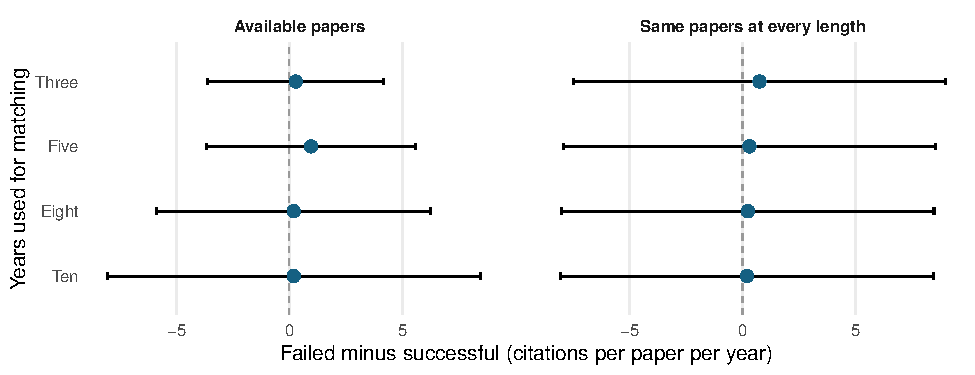
\includegraphics[width=\linewidth]{matching_history.pdf}
\caption{Sensitivity to matching-history length. Points show failed-minus-successful matched changes; bars are 95\% paper/report clustered intervals conditional on matches. The left panel uses available papers at each length; the right uses the same \CommonHistoryN{} originals, with controls reselected. Panels share an axis and outcome window: the last three pre-report years versus the first three post-report years.}
\label{fig:history}
\end{figure}

Pre-fit can look good because it was optimized. We therefore select controls using the earlier years of each five-, eight-, or ten-year history and reserve the final two pre-report years for validation. The five-year check fits on years minus five through minus three and evaluates years minus two and minus one. No post-report citation count enters selection. Table~\ref{tab:validation} reports the held-out level gap and difference in changes. Unlike the older pre-window diagnostic in Table~\ref{tab:diagnostics}, this exercise trains new matches and evaluates later pre-period observations. Both condition on the completed-comparison sample. Neither is independent confirmation or proof of parallel trends; early disclosure could contaminate the final pre-report years. We do not select papers by whether a pre-trend test rejects.

\begin{table}[H]
\centering
\caption{Prediction of pre-report citations outside the matching period.}
\label{tab:validation}
\small
\begin{tabular}{llrrr}
\toprule
History & Outcome & Originals & Level gap & Change gap \\
\midrule
5 years & Failed & 112 & $+8.53$ & $+1.56$ \\
5 years & Successful & 115 & $+18.55$ & $+0.66$ \\
8 years & Failed & 50 & $+13.65$ & $+0.04$ \\
8 years & Successful & 59 & $+30.73$ & $-0.59$ \\
10 years & Failed & 39 & $+15.24$ & $+0.56$ \\
10 years & Successful & 43 & $+41.17$ & $-0.93$ \\
\bottomrule
\end{tabular}

\par\smallskip\begin{minipage}{\linewidth}\footnotesize
Controls are reselected without the last two pre-report years. The level gap is the original-minus-control mean over those years. The change gap is the original-minus-control difference in the one-year change between them. Units are annual citations per paper. These descriptive diagnostics have no inferential intervals and condition on the available sample at each history length.
\end{minipage}
\end{table}

\subsection{Define the pool before choosing the nearest papers}
The preferred pool is the full set of research papers of the same indexed publication year, journal, and article type as each original. This holds publication age and venue approximately fixed and subjects controls to the same calendar years. Publisher dates establish that papers existed before the baseline. The present random sample of twenty candidates is a computational shortcut, not the definition of an appropriate counterfactual. The next collection should enumerate the full pool, acquire histories, and then select controls. Adding history cannot recover a close match omitted from the pool.

Assessed and unassessed papers can differ in visibility, topic, and expected replicability. Matching must be evaluated on prior citation levels and changes. Topic restrictions based on the original published text are a possible sensitivity; later citations, later journal impact, and responses to the replication are inappropriate matching variables. For expanded pools, we propose an overlap restriction: the original must lie inside the pool's annual citation range in every matching year. Report excluded originals separately and compare this restricted population with the unrestricted pool. This coordinate-wise rule does not guarantee a close joint trajectory, so held-out prediction errors still matter. Freeze any additional distance caliper using pre-period prediction before estimating post-period contrasts in the expanded sample.

If the full same-journal/year pool lacks support, report that limitation. A separate alternative can broaden publication year within the journal or use field/year peers in other journals, but requires adjustment for publication age or venue. We should not widen the pool until a preferred post-report answer appears.

The current implementation excludes every known assessed paper and papers currently marked retracted. The preferred longitudinal pool instead records dated replication, reproduction, and retraction events. A control must be unexposed at the focal report date and contributes only through years before its own exposure. A conservative sensitivity uses controls unassessed throughout the outcome window. Current retraction flags and exclusion of every eventual assessment condition eligibility on events after some focal reports. Those retrospective exclusions remain in this snapshot; dated risk-set construction and full-pool collection are not completed analyses.

\subsection{Estimation and causal interpretation}
The primary estimator is a matched difference in differences, with separate averages for successful and failed outcomes and equal weight per original. An unmatched same-journal/year comparison should accompany expanded collection so the consequences of matching are visible. Neither matching nor fixed effects establishes parallel trends.

With dated exposures and larger pools, a cohort-specific event study can estimate each lead and lag and aggregate with explicit original-paper weights. Group-time estimators allow never-assessed or not-yet-assessed controls without using already assessed papers as untreated comparisons \citep{callaway2021}. Cohort-interacted event studies are another established option \citep{sun2021}. A pooled two-way fixed-effects regression that uses earlier-treated papers as controls for later-treated papers is not proposed. The current within-comparison change estimator does not make those comparisons.

Synthetic difference in differences is a secondary candidate for cohorts with long, balanced histories and enough controls \citep{arkhangelsky2021}. Standard synthetic DiD fits unit weights using pre-treatment trajectories and time weights using control outcomes before and after treatment. Pre-period placebo exercises can assess the procedure without using treated post-period outcomes to choose it. Its block-treatment implementation requires common onset within each fitted cohort. Concatenating staggered reports as simultaneous would change the design. Good fit and placebo ranks would not establish random assignment.

The event should ultimately be the earliest verified public release of an assessment, with journal publication analyzed separately. Where first disclosure cannot be established, the journal-date analysis must remain labeled accordingly. Later reports and author responses should be dated, with censoring treated as a change in the estimand.

Causal interpretation requires credible untreated comparisons, no anticipation, and no differential shocks to citation growth. Topic-wide attention and selection of unusually visible papers for replication are plausible violations. The held-out gaps and poor level matches give reasons for caution. Completing pools, dating exposures, and reporting longer paths are prerequisites for stronger interpretation, not guarantees of it. Inference should retain dependence from reused papers and shared reports; current intervals condition on matches and labels and exclude uncertainty about disclosure dates and design selection.

\end{document}
